\documentclass[
	letterpaper, % Paper size, specify a4paper (A4) or letterpaper (US letter)
	10pt, % Default font size, specify 10pt, 11pt or 12pt
]{CSUniSchoolLabReport}

\usepackage{fancyvrb}
\usepackage{multicol}
\usepackage{subcaption}
\captionsetup[subfigure]{labelformat=empty}


\title{Analyzing current vs voltage relation in resistors, potentiometers and lightbulbs}

\author{Sebastien \textsc{Psarianos}\\ Sofiya \textsc{P'yavka}}

\date{\today}

\begin{document}

\setlength\arrayrulewidth{2pt}

\maketitle

\section{Introduction}
The objective of this experiment was to determine the charge to mass ratio of an
electron. An electron moving in a magnetic field will experience a force of:
$$F=e\vec v\times \vec B$$
$e$ is the charge of the electron, $v$ is its velocity and $B$ is the magnetic field.
Using Newton’s second law of motion, this can be further written in terms of $F = ma = m\frac{v^2}{r}=evB$ where $r$ is the radius of
the circular orbit that the electron will follow and $m$ is its mass. The electron will
be accelerated through a potential difference in this experiment and the curvature
of the path can be described using:
$$\frac{1}{r}= \frac{B}{\sqrt V}\sqrt{\frac{e}{2m}}$$
$V$ is the potential difference. The magnetic field acting on the electron is a
sum of the external magnetic field from outside sources and the field due to the
coils. Thus the total field acting on the electron is:
$$B=B_C+B_e = \left(\frac{4}{5}\right)^{\frac{3}{2}} \frac{\mu_0nI}{R} + \frac{\sqrt 2 R }{\mu_0n}\left(\frac{5}{4}\right)^{\frac{3}{2}}$$
$I_0$ is a constant proportional to the external magnetic field, $\mu_0$ is defined in the appendix as \textbf{Constant 1},
$R$ is the radius of the coils and $n$ is the number of turns in each coil. Thus, this
equation can be subbed into the equation describing the curvature of the electron path to obtain
$$\frac{1}{r}=k\frac{I-I_0}{\sqrt V}\sqrt{\frac{e}{m}}$$
\begin{center}
	\textbf{Equation 1: Electron path model}
\end{center}
From this one can determine the experimental value of the charge to mass ratio of an electron.
\section{Procedure and Methodology}
The experimental apparatus as pictured in \textbf{Figure 1} consisted of a lightbulb containing hydrogen gas
and an electron gun. The electrons were accelerated through an anode connected to a power source
which varies between $0-300 V$ and a voltmeter which was set to $1000 V$. This was connected in a circuit
with two Helmholtz coils whose current was provided by an $8V$ power supply in series with an ammeter
which was set to $3 A$ and a rheostat. To determine the radius of one Helmholz coil, the diameter was
measured using a ruler and the number of turns in the coils was indicated on the apparatus.\\

\begin{figure}[H]
	\begin{subfigure}{\textwidth}
		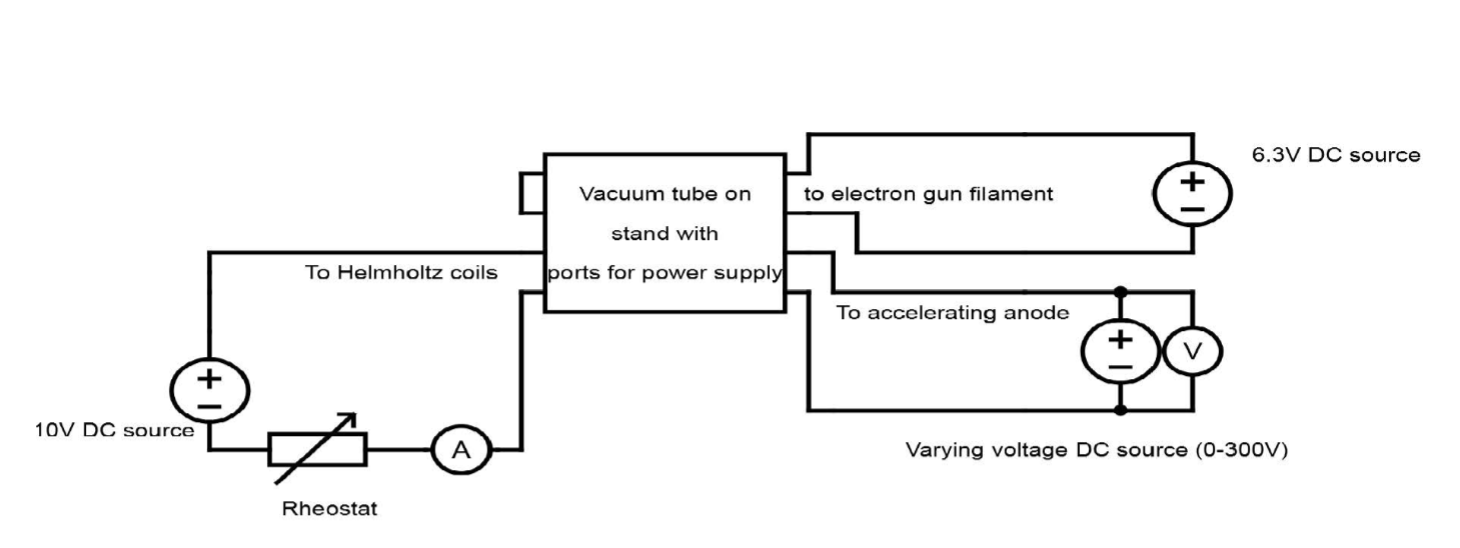
\includegraphics[width=\textwidth]{../figures/apparatus.png}
		\caption{\textbf{Figure 1: Apparatus Schematic}}
	\end{subfigure}
\end{figure}

\textbf{Experiment 1}: The $0-300 V$ power supply and then the $8 V$ power supply were turned on.
The measurements of the diameter of the paths first began by fixing the $0-300 V$ power supply
voltage to a value of $149.820 V \pm 0.009$. The current was varied using the rheostat for ten values
incremented by $0.1 A$ from $1-2 A$, each measured using the ammeter. For each current measurement,
the diameter of the electron path was measured using a self-illuminated scale and plastic
reflector and recorded. This procedure was repeated another time for values within a
similar range of each increment.\\

\textbf{Experiment 2}: Similarly, the same procedure outlined above was repeated, however the
current was fixed to a value of $1.511\pm 0.003 A$ using the rheostat. The voltage was then varied by
increments of $10 V$ from $200-300 V$ and measured using the voltmeter. The diameter of the
electron beam path was measured and the procedure was repeated for a second time for values
within a similar range of each increment.\\

Note all the measurements were recorded in a Google Sheet and the voltmeter and ammeter were Keysight 34461A multimeters.\\
\section{Results}
Note, all referenced functions, equations and constants can be found in the appendix.\\

To determine the experimental value of the external magnetic field, the model as implemented by \textbf{Function 3}
was defined. An array of coil field values was first determined using \textbf{Equation 2}, passing in the varied
current data. The radius of the two coils was determined using a ruler to be $31.1 \pm 0.1 cm$. Since the markings
on the ruler were a bit faded, an uncertainty of $0.05 cm$ for either end of the measured section was used.
The number of turns was indicated on the apparatus and $\mu_0$ (Vacuum Permeability) is a constant defined in the
appendix (\textbf{Constant 1}). \textbf{Function 3} (implementation of \textbf{Equation 6}) was passed into scipy's \lstinline{curve_fit} function and was fitted to the coil field
and current data. The magnitude of the external magnetic field was determined to be $0.00011 \pm 0.00002 T$.
The uncertainty was determined using \lstinline{curve_fit}'s covariance values since the diagonals of the covariance
matrix represent the variability of each parameter and the square root of this was taken to calculate the
standard error. \textbf{Figure 2} demonstrates the linear relationship between the coil's field and the current where
the y-intercept represents the value of the external field. \textbf{Figure 3} is the corresponding residuals plot for \textbf{Figure 2}. \\

\begin{figure}[H]
	\begin{subfigure}{0.45\textwidth}
		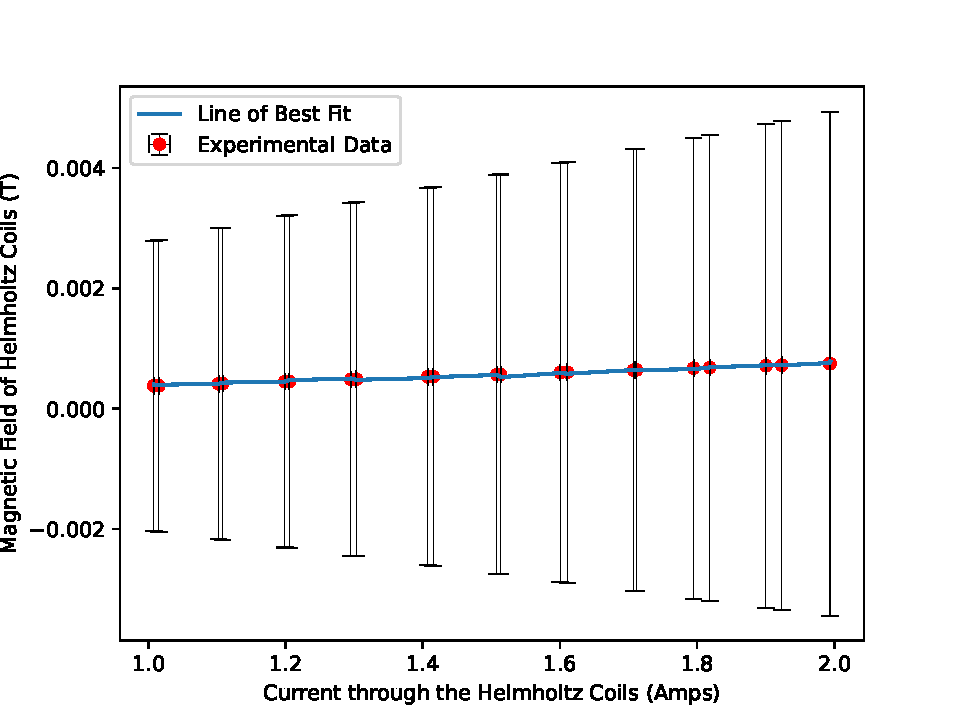
\includegraphics[width=\textwidth]{../figures/externalMagneticGraph.pdf}
		\caption{\textbf{Figure 2: Graph of fit used to determine the coil field}}
	\end{subfigure}
	\hspace*{\fill}
	\begin{subfigure}{0.45\textwidth}
		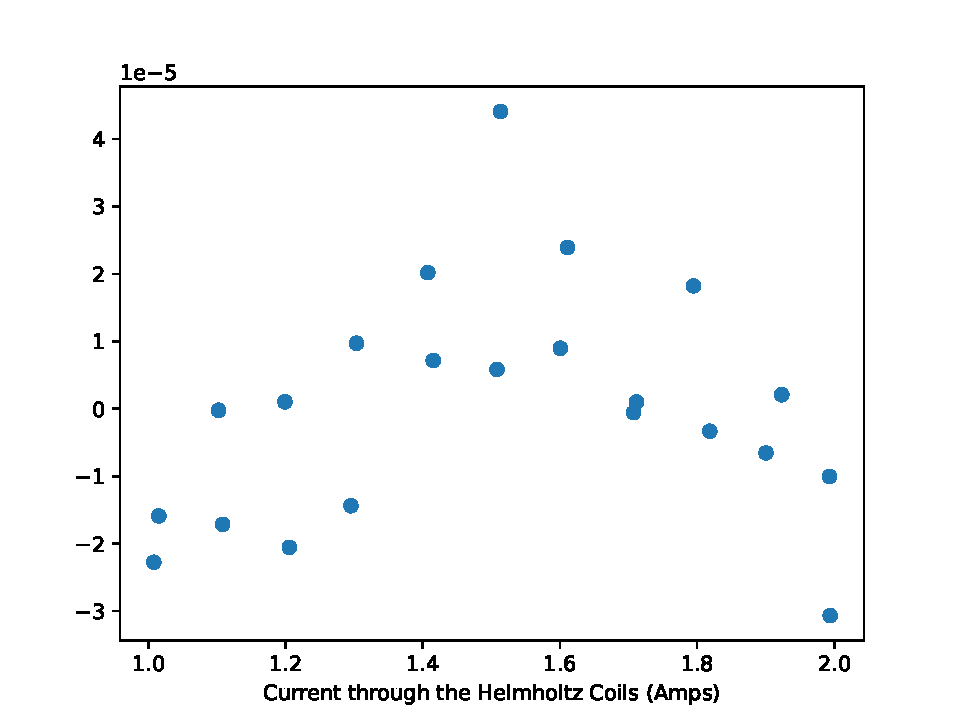
\includegraphics[width=\textwidth]{../figures/externalMagneticResiduals.pdf}
		\caption{\textbf{Figure 3: Residuals of coil field fit}}
	\end{subfigure}
\end{figure}


The experimental values of the charge to mass ratios were then determined using the models as defined by \textbf{Function 1} and \textbf{Function 2}.
The experimental value of the external field was used in both models. Both models were passed into scipy's \lstinline{curve_fit} where \textbf{Function 1} was
fitted to the current data and its corresponding electron path radius data and \textbf{Function 2} was fitted to the voltage data and its corresponding electron
path radius data. Note, to determine the radius data, the collected diameter data was divided by 2. The final values were determined to be $250000000000 \pm 9700000000 C/kg$
and $180000000000 \pm 900000000 C/kg$ respectively. Note the parameters of best fit had to be squared. Similarly to the external field, the uncertainty
in the values was determined using \lstinline{curve_fit}'s covariance values, the same technique as before was used to get the standard error from the
covariance matrix. The value was propagated as the final value was squared using \textbf{Equation 5}. \textbf{Figures 4 and 5} demonstrate the relationship between the
current and the radius of the electron beam and the voltage and the radius of the electron beam respectively.\\

\begin{figure}[H]
	\begin{subfigure}{0.45\textwidth}
		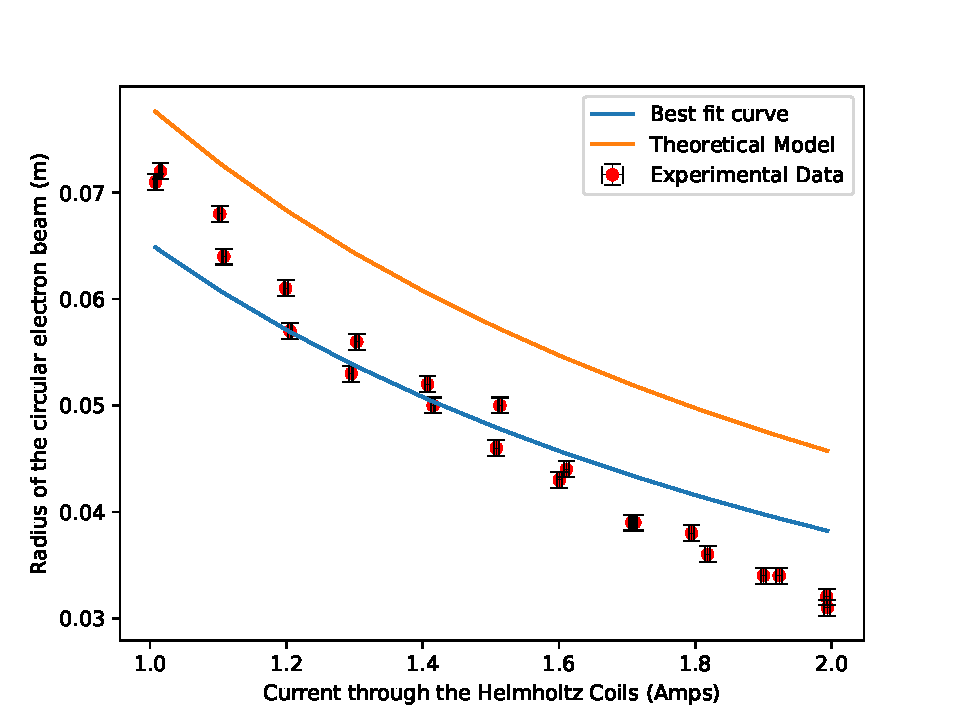
\includegraphics[width=\textwidth]{../figures/variedCurrentGraph.pdf}
		\caption{\textbf{Figure 4: Experiment 1 data plot of electron path radius vs current through the Helmholtz coils. Includes best fit curve, error bars and the theoretical model where the literature charge mass ratio was used}}
	\end{subfigure}
	\hspace*{\fill}
	\begin{subfigure}{0.45\textwidth}
		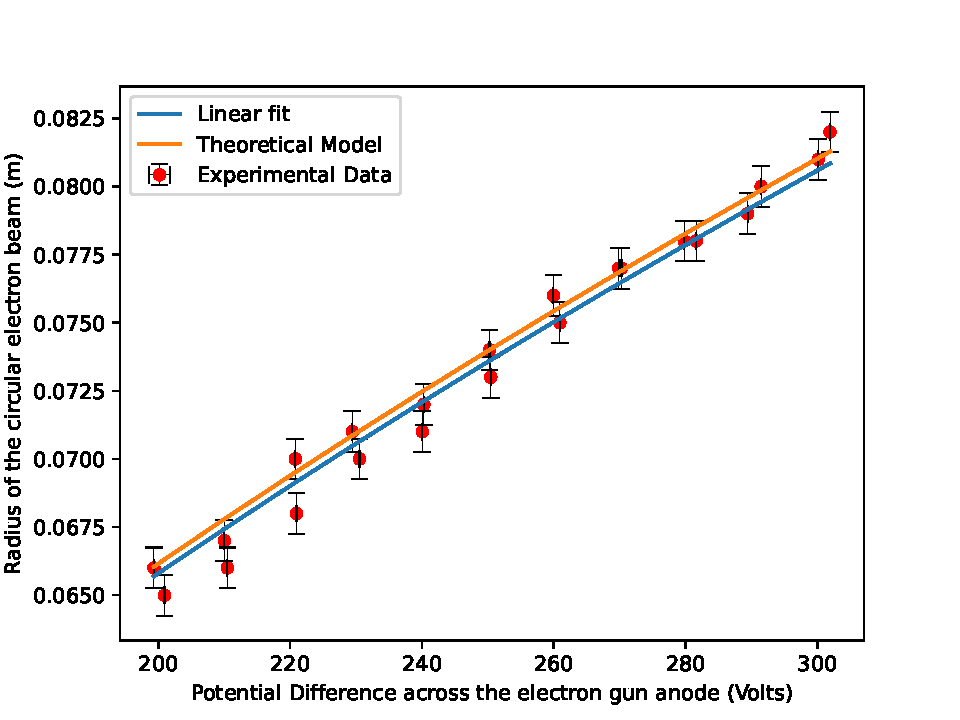
\includegraphics[width=\textwidth]{../figures/variedVoltageGraph.pdf}
		\caption{\textbf{Figure 5: Experiment 2 data plot of electron path radius vs potential difference across the electron gun anode. Includes best fit curve, error bars and the theoretical model where the literature charge mass ratio was used}}
	\end{subfigure}
	\begin{subfigure}{0.45\textwidth}
		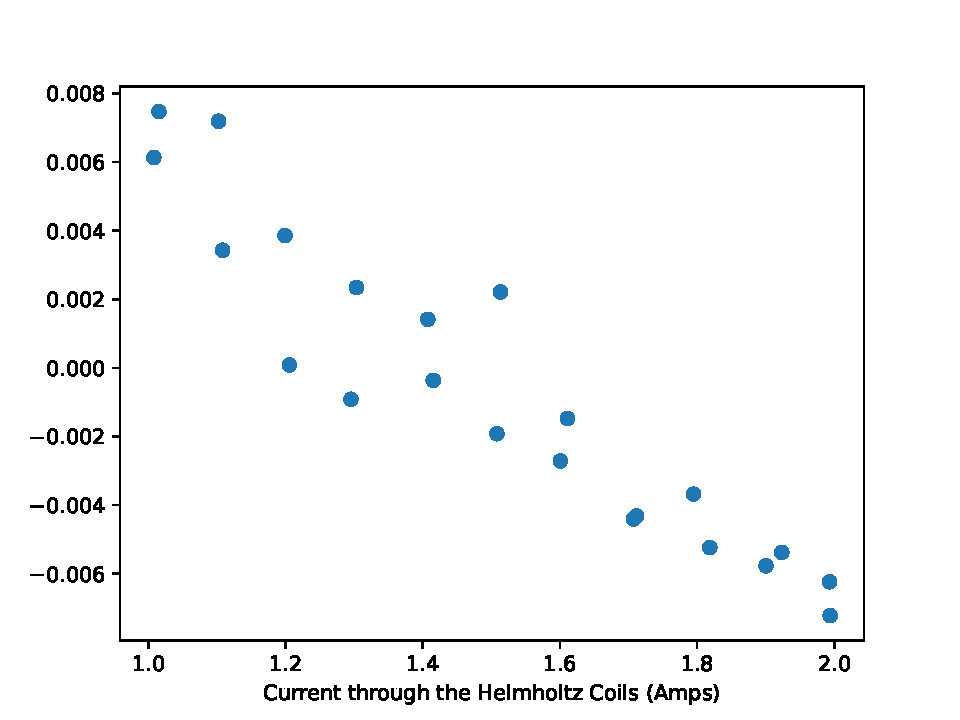
\includegraphics[width=\textwidth]{../figures/variedCurrentResiduals.pdf}
		\caption{\textbf{Figure 6: Experiment 1 residual plot}}
	\end{subfigure}\qquad\quad
	\begin{subfigure}{0.45\textwidth}
		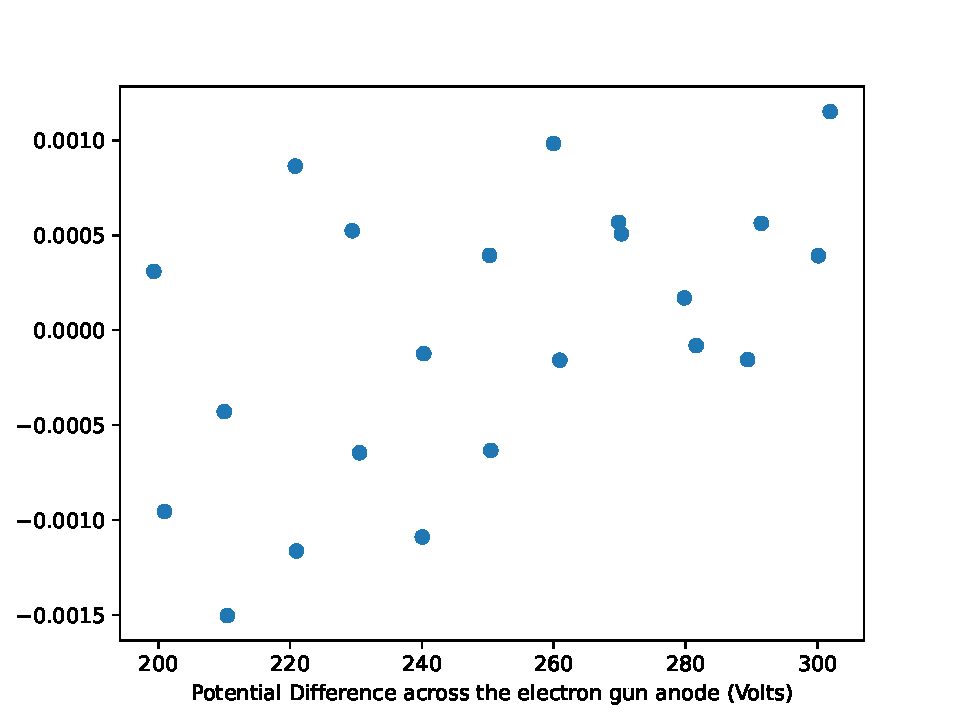
\includegraphics[width=\textwidth]{../figures/variedVoltageResiduals.pdf}
		\caption{\textbf{Figure 7: Experiment 2 residual plot}}
	\end{subfigure}
\end{figure}

Note the current and voltage uncertainties were determined from the Keysight 34461A multimeter manual
and were implemented using \textbf{Function 4}. An uncertainty of  $3 * 0.05 cm$ was used as the
uncertainty of the diameters of the electron beam paths due to measurements being taken on
either side and the middle section of the self-illuminated scale. The self-illuminated
scale and plastic reflector were used instead of a traditional ruler to eliminate problems of
parallax. When a measurer uses the scale, the scale and reflector work to “project” the scale
onto the electron beam path so that it seems like the scale is as close to the beam as possible.
Thus viewing the beam from a different angle will not cause much discrepancy in the measured values.\\

Lastly the reduced chi-squared values determined for the varied current model and varied voltage model were \
$36.47$ and $0.97$ respectively using \textbf{Function 4}.

\section{Analysis and Discussion}
Throughout the experiment the electrons consistently followed the predicted circular path. Consider
$\frac 1r = \frac B {\sqrt V} \sqrt{\frac{e}{2m}}$, rearranging the equation for $r$,
$r = \frac{\sqrt V}{B}\sqrt{\frac{2m}{e}}$. As $V\rightarrow 0$ and $B\rightarrow \infty$,
$r\rightarrow 0$ and thus the electron's circular path becomes arbitrarily small. It follows
that measuring the radius of the electrons' path in this case becomes more difficult as the
trajectory becomes smaller, introducing the likelihood of greater error within the measurements.
One way to reduce error, and this applies to trajectories of any radius, is to use a computer
program which takes images of the circular electron beam and uses a scale to obtain precise
measurements of the radius instead of using the self-illuminated scale and plastic reflector.
This would also help to eliminate/reduce the effects of parallax on the obtained measured values.\\

The magnitude of the final value determined for the external magnetic field was approximately
$0.00011 \pm 0.00002 T$ which is close to the ideal value of $0 T$ for a perfect experimental
set up where no external field exists. Although an external magnetic field was present, other
ferromagnetic materials and objects which generate magnetic fields such as cellphones did not
noticeably affect the trajectory of the electrons when held close to the bulb. The Earth’s magnetic
field is approximately $25000-65000 nT < 0.00011 \pm 0.00002 T$, thus the experimental value
indicates other sources contributed to the external magnetic field such as the building and other
devices/instruments (“Geomagnetism Frequently Asked Questions”).\\

The final experimental values determined for the electron charge to mass ratios from the varied
current and voltage data were $250000000000 \pm 9700000000 C/kg$ and $180000000000 \pm 900000000 C/kg$
and the reduced chi-squared values were $36.47$ and $0.97$ respectively. In comparison, the theoretical
value rounded to two significant figures is $180000000000 C/kg$. The experimental value determined
from the data collected using a fixed value of current agrees with the theoretical value but although
the order of magnitude is correct, the theoretical value does not fall within the range of the experimental
value determined from the data collected using a fixed value of voltage. However, during the experiment
the current reading on the ammeter significantly fluctuated which likely resulted in greater
measurement error. Error may have also resulted from the actual measurement process as a better placement
of the self-illuminated scale and plastic reflector was determined when data was being collected for a
fixed value of current. In regards to the reduced chi-squared values determined, the value $0.97$ corresponding to
data collected using a fixed current indicates that the corresponding model used is a good fit for the experimental
data and examining the line of best fit in \textbf{Figure 5}, it is close to the theoretical line. In contrast, the reduced
chi-squared value of $36.47$ corresponding to data collected using a fixed voltage indicates that the model is
ill-fitting for the experimental data and examining the curve of best fit in \textbf{Figure 4}, it is quite far from the
theoretical curve. As stated earlier, error likely came from the experimental measurements. \textbf{Figure 6 and 7} are the residual plots for \textbf{Figures 4 and 5} respectively.

\section{Conclusion}
Although the experimental value determined from the data collected using a fixed value of voltage deviates away from
the theoretical electron charge to mass ratio, this was likely due to measurement errors. In contrast, the experimental
value determined from the data collected using a fixed value of current agrees with the theoretical value and thus verifies
that the charge to mass ratio of an electron can be quantified using Newton's second law of motion.

\section{References}
National Oceanic and Atmospheric Administration. (n.d.). Geomagnetism \\
\null\qquad Frequently Asked Questions.\\
\null\qquad National Centers for Environmental Information. Retrieved November 1, 2022,
\null\qquad from \\
\null\qquad\lstinline{https://www.ngdc.noaa.gov/geomag/faqgeom.shtml#:~:}\\
\null\qquad\lstinline{text=The%20Earth's%20magnetic%20field%20intensity}.\\
\null\qquad\lstinline{magnetic%20north%20and%20true%20north}.\\\\
\newpage
\section{Appendix}
{\Large\textbf{Constants}}\\
\begin{tabular}{p{0.45\linewidth} p{0.45\linewidth}}

$$ \mu_0= 4\pi \cdot 10^{-7}WbA^{-1}m^{-1}$$
\begin{center}
	\textbf{Constant 1: Vacuum Permeability}
\end{center}
&
$$k=\frac{1}{\sqrt 2}\left(\frac{4}{5}\right)^{\frac{3}{2}}\frac{\mu_0n}{R}$$
\begin{center}
	\textbf{Constant 2: $k$ constant}
\end{center}
\end{tabular}\\\\
{\Large\textbf{Equations}}\\
\begin{tabular}{p{0.45\linewidth} p{0.45\linewidth}}

$$\frac{1}{r}=k\frac{I-I_0}{\sqrt V}\sqrt{\frac{e}{m}}$$
\begin{center}
	\textbf{Equation 1: Electron path model}
\end{center}
&
$$B_c = \left(\frac45\right)^{\frac32} \frac{\mu_0nI}{R}$$
\begin{center}
	\textbf{Equation 2: Coil magnetic field model}
\end{center}
\\
$$ u(x) = \pm\left|\frac{xp_v}{100} + \frac{rp_r}{100}\right|$$
\begin{center}
	\textbf{Equation 3: Multimeter uncertainty calculation formula}
\end{center}
&
$$\chi^2_R = \frac{1}{N-n}\sum_{i=1}^N\left(\frac{y_i-y(x_i)}{u(y_i)}\right)$$
\begin{center}
	\textbf{Equation 4: Reduced chi-Squared Metric}
\end{center}\\
$$u(x^2) = 2xu(x)$$
\begin{center}
	\textbf{Equation 5: Squared value error propagation}
\end{center}
&
$$B_c =\frac 1r \sqrt{\frac{2m}{e}} \sqrt V  - B_e$$
\begin{center}
	\textbf{Equation 6: Relation between radius, background field and coil field}
\end{center}
\end{tabular}\\

\newpage
{\Large\textbf{Python Functions}}
\begin{verbatim}
def variedCurrent(I, a):
    return 1 / (a * k * ((I - externalFitVariables[1] / k) / np.sqrt(149.820)))
\end{verbatim}
\begin{center}
		\textbf{Function 1: Electron path model with constant voltage set to 149.820 Volts}
	\end{center}
\begin{verbatim}
def variedVoltage(v, a):
    return 1 / (a * k * ((1.510946 - externalFitVariables[1] / k) / np.sqrt(v)))
\end{verbatim}
\begin{center}
	\textbf{Function 2: Electron path model with constant current set to 1.510946 Amps}
\end{center}
\begin{verbatim}
def externalField(r, b, B):
    return b * np.sqrt(149.820) / r - B
\end{verbatim}
\begin{center}
	\textbf{Function 3: Coil magnetic field model (implements Equation 6)}
\end{center}
\begin{verbatim}
def multimeterUncertainty(value, valuePercentage, range, rangePercentage):
    return (value * valuePercentage + range * rangePercentage) / 100
\end{verbatim}
\begin{center}
	\textbf{Function 4: Function used to calculate uncertainty for the multimeter (implements Equation 3)}
\end{center}

\begin{verbatim}
def reducedChiSquared(x, y, yerr, model, modelParams):
    return (
        1
        / (len(y) - len(modelParams))
        * np.sum(((y - model(x, *modelParams)) / yerr) ** 2)
    )
\end{verbatim}
\begin{center}
	\textbf{Function 5: Function used to calculate reduced chi-squared values (implements Equation 4)}
\end{center}

\newpage
{\Large\textbf{Raw data tables}}
\begin{figure}[H]
	\begin{subfigure}{0.45\textwidth}
		\begin{tabular}{|p{0.45\textwidth} | p{0.45\textwidth} | }
\hline
Current through Helmholtz coil (A) & Measured electron path radius (m)\\
\hline
1.0078$\pm$0.002&0.071$\pm$0.0008\\
1.015223$\pm$0.002&0.072$\pm$0.0008\\
1.10219$\pm$0.003&0.068$\pm$0.0008\\
1.10813$\pm$0.003&0.064$\pm$0.0008\\
1.199013$\pm$0.003&0.061$\pm$0.0008\\
1.205404$\pm$0.003&0.057$\pm$0.0008\\
1.29518$\pm$0.003&0.053$\pm$0.0008\\
1.303277$\pm$0.003&0.056$\pm$0.0008\\
1.40726$\pm$0.003&0.052$\pm$0.0008\\
1.415226$\pm$0.003&0.050$\pm$0.0008\\
1.508114$\pm$0.003&0.046$\pm$0.0008\\
1.513418$\pm$0.003&0.050$\pm$0.0008\\
1.600502$\pm$0.003&0.043$\pm$0.0008\\
1.61092$\pm$0.003&0.044$\pm$0.0008\\
1.70728$\pm$0.004&0.039$\pm$0.0008\\
1.711507$\pm$0.004&0.039$\pm$0.0008\\
1.794713$\pm$0.004&0.038$\pm$0.0008\\
1.818418$\pm$0.004&0.036$\pm$0.0008\\
1.900371$\pm$0.004&0.034$\pm$0.0008\\
1.923341$\pm$0.004&0.034$\pm$0.0008\\
1.993017$\pm$0.004&0.032$\pm$0.0008\\
1.993969$\pm$0.004&0.031$\pm$0.0008\\
\hline
\end{tabular}

		\caption{\textbf{Table 1: Experiment 1 raw data: Varied current with constant anode voltage of 149.820V}}
	\end{subfigure}
	\hspace*{\fill}
	\begin{subfigure}{0.45\textwidth}
		\begin{tabular}{|p{0.45\textwidth} | p{0.45\textwidth} | }
\hline
Electron gun anode voltage (V) & Measured electron path radius (m)\\
\hline
199.334$\pm$0.01&0.066$\pm$0.0008\\
200.944$\pm$0.01&0.065$\pm$0.0008\\
210.022$\pm$0.01&0.067$\pm$0.0008\\
210.484$\pm$0.01&0.066$\pm$0.0008\\
220.791$\pm$0.01&0.070$\pm$0.0008\\
220.961$\pm$0.01&0.068$\pm$0.0008\\
229.437$\pm$0.01&0.071$\pm$0.0008\\
230.539$\pm$0.01&0.070$\pm$0.0008\\
240.056$\pm$0.01&0.071$\pm$0.0008\\
240.284$\pm$0.01&0.072$\pm$0.0008\\
250.261$\pm$0.01&0.074$\pm$0.0008\\
250.449$\pm$0.01&0.073$\pm$0.0008\\
259.95$\pm$0.01&0.076$\pm$0.0008\\
260.929$\pm$0.01&0.075$\pm$0.0008\\
269.85$\pm$0.01&0.077$\pm$0.0008\\
270.277$\pm$0.01&0.077$\pm$0.0008\\
279.812$\pm$0.01&0.078$\pm$0.0008\\
281.619$\pm$0.01&0.078$\pm$0.0008\\
289.422$\pm$0.01&0.079$\pm$0.0008\\
291.487$\pm$0.01&0.080$\pm$0.0008\\
300.142$\pm$0.01&0.081$\pm$0.0008\\
301.939$\pm$0.01&0.082$\pm$0.0008\\
\hline
\end{tabular}

		\caption{\textbf{Table 2: Experiment 2 raw data: Varied voltage with constant coil current of 1.510946A}}
	\end{subfigure}
\end{figure}
\newpage
{\large\textbf{Sample Calculations}}\\
This calculation is based on \textbf{Equation 3}\\
$p_V=0.002$, $r=1000$, $p_r=0.0006$ (from the Keysight manual)\\
Let $V_i$ represent an arbitrary voltage measurement made with the $1000V$ setting.\\
$$ u(V_i) = \pm\left|\frac{0.002V_i}{100} + \frac{1000 \times 0.0006}{100}\right| = \pm\left|2\times 10^{-5}V_i+0.006\right|$$
For example in table, the first measured voltage was: $V_1=199.334V$\\
$$ u(V_1) = \pm\left|2\times 10^{-5} \times 199.334V + 0.006\right| \approx \pm 0.00999$$
\begin{center}
    \textbf{Calculation 1: Voltmeter Calculation sample for $1000V$ setting}\\
\end{center}

\vspace{10pt}
This calculation is based on \textbf{Equation 3}:\\
$p_V=0.18$, $r=3$, $p_r=0.02$ (from the Keysight manual)\\
Let $I_i$ represent an arbitrary current measurement made with the $3A$ setting.\\
$$u(I_i) = \pm\left|\frac{0.18I_i}{100} + \frac{3 \times 0.02}{100}\right| = \pm\left|1.8\times10^{-3}I_i + 0.0006\right|$$
For example in table one, the first measured current was: $I_1 = 1.0078A$.
$$ u(I_1) = \pm\left|1.8\times10^{-3}\times1.0078 + 0.0006\right|\approx \pm 0.0024$$
\begin{center}
    \textbf{Calculation 2: Ammeter Calculation sample for $3A$ setting}
\end{center}
In practice all calculations were done using the python implementation of \textbf{Equation 3}, \textbf{Function 4}.
\end{document}